\documentclass[10pt]{beamer}
\usepackage[english]{babel}
\usepackage[utf8]{inputenc}
\usepackage[T1]{fontenc}
\usepackage{helvet}
\usepackage{lipsum}  
\usepackage{graphicx,subfigure}
%-------------------------------------------------------
% INFORMATION IN THE TITLE PAGE
%-------------------------------------------------------

\newcommand{\cstitle}{\textbf{Prediction of peptide MHC binding and	presentation using transformers and transfer learning in cancer immunology context}
\subtitle[]{Tésis de doctorado}}
\newcommand{\cscourseCode}{IFI TC3 Doctoral Consortium}
\newcommand{\csauthor}{MSc. Vicente Machaca Arceda}
\institute[UNSA]{Universidad La Salle}
\newcommand{\csemail}{vmachaca@utec.edu.pe}
\newcommand{\instituteabr}{UTEC}
\newcommand{\nameUp}{}
\date{2023}
\title[\cscourseCode]{\cstitle}
\author{\csauthor}
%%%%%%%%%%%%%%%%%

%-------------------------------------------------------
% CHOOSE THE THEME
%-------------------------------------------------------
\def\mycmd{0} % UNSA
\def\mycmd{1} % SALLE
%\def\mycmd{2} % UTEC
%-------------------------------------------------------

\if\mycmd0
\usepackage{csformat}
\newcommand{\chref}[3][blue]{\href{#2}{\color{#1}{#3}}}%

\fi

\if\mycmd1
\usetheme[]{Feather}
\newcommand{\chref}[2]{	\href{#1}{{\usebeamercolor[bg]{Feather}#2}} }
\fi

\if\mycmd2
\usetheme{UTEC2020}	
\newcommand{\chref}[3][blue]{\href{#2}{\color{#1}{#3}}}%
\fi

\newcommand{\1}{
	\setbeamertemplate{background}{
		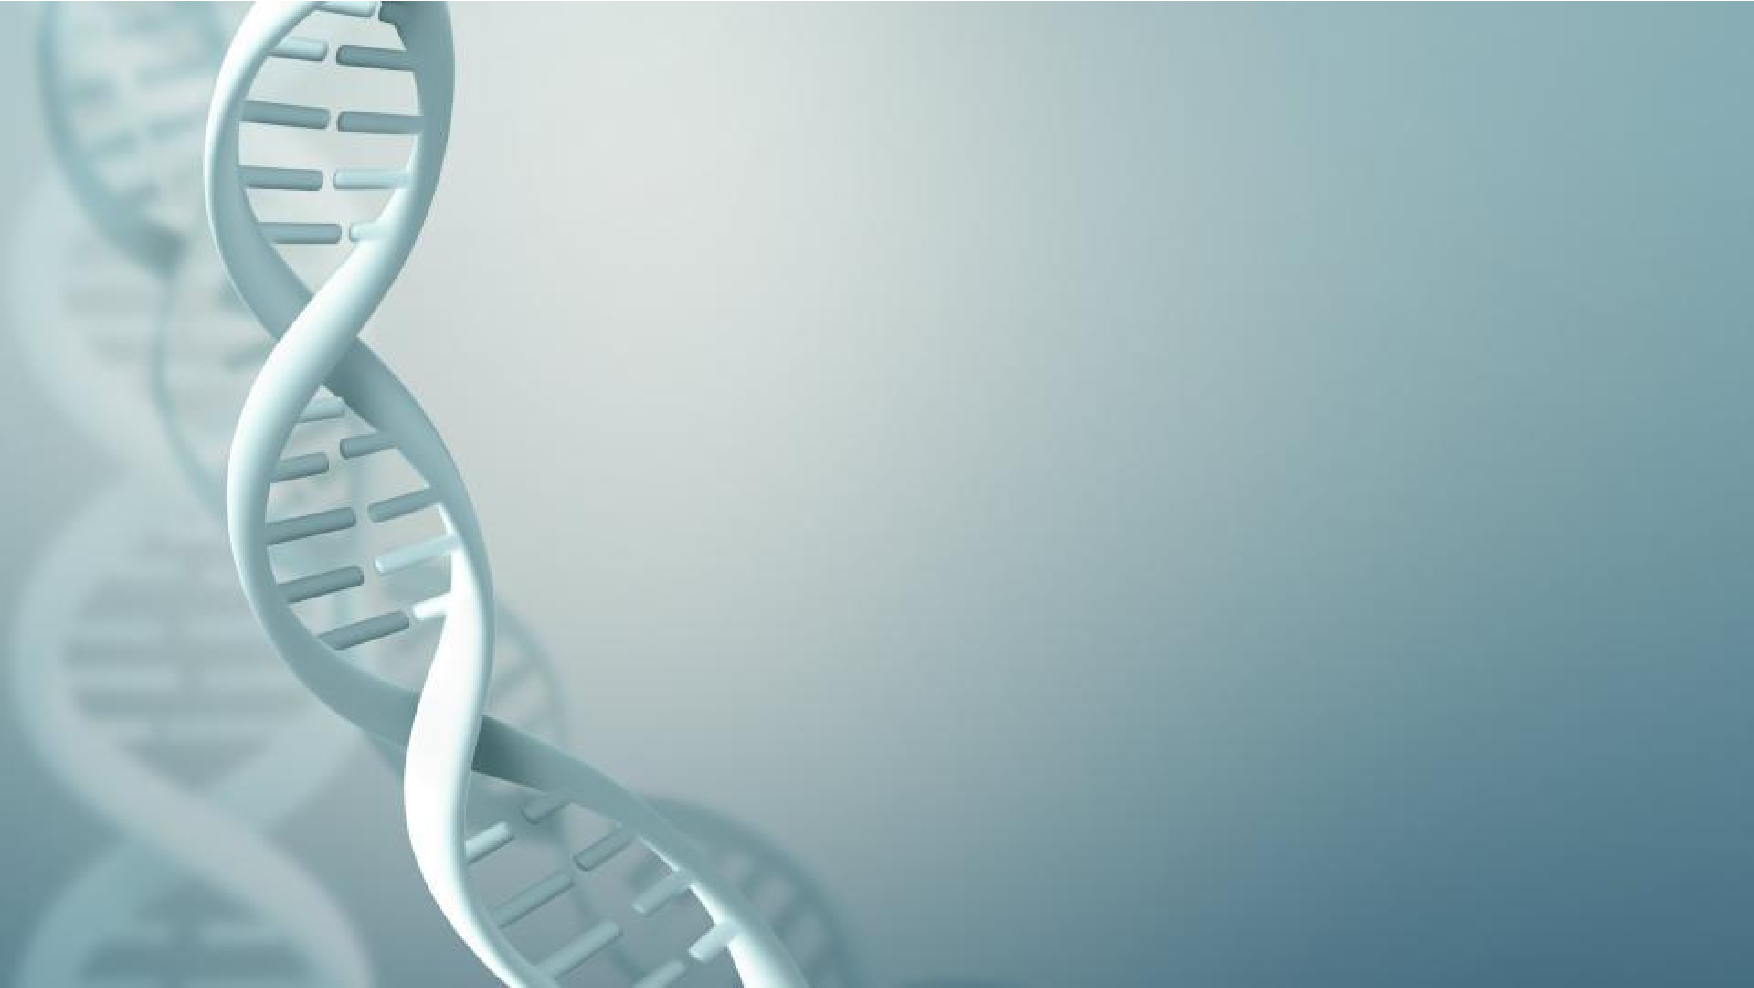
\includegraphics[width=\paperwidth,height=\paperheight]{img/1}
		\tikz[overlay] \fill[fill opacity=0.75,fill=white] (0,0) rectangle (-\paperwidth,\paperheight);
	}
}



%-------------------------------------------------------
% THE BODY OF THE PRESENTATION
%-------------------------------------------------------

\begin{document}
	
	
	\AtBeginSubsection[]
	{
		\begin{frame}
			\frametitle{Content}
			\tableofcontents[currentsubsection]
		\end{frame}
	}
	
	
	%-------------------------------------------------------
	% THE TITLEPAGE
	%-------------------------------------------------------
	
	\if\mycmd0
	\maketitle
	\fi
	
	\if\mycmd1 % MY THEME
	\1{
		\begin{frame}[plain,noframenumbering] 
			\titlepage 
	\end{frame}}
	\fi
	
	\if\mycmd2
	\begin{frame}
		\titlepage
	\end{frame}
	\fi
	%-------------------------------------------------------
	%-------------------------------------------------------


%-------------------------------------------------------
%-------------------------------------------------------
\begin{frame}{Content}
	\tableofcontents
\end{frame}
%-------------------------------------------------------
%-------------------------------------------------------


%%%%%%%%%%%%%%%%%%%%%%%%%%%%%%%%%%%%%%%%%%%%%%%%%%%%%%%%%%%%%%%%%%%%%%%%%%%%%%%%%%%%%%%%%%%%%%%%%%%%%%%%%%%%%%%%
%%%%%%%%%%%%%%%%%%%%%%%%%%%%%%%%%%%%%%%%%%%%%%%%%%%%%%%%%%%%%%%%%%%%%%%%%%%%%%%%%%%%%%%%%%%%%%%%%%%%%%%%%%%%%%%%
%%%%%%%%%%%%%%%%%%%%%%%%%%%%%%%%%%%%%%%%%%%%%%%%%%%%%%%%%%%%%%%%%%%%%%%%%%%%%%%%%%%%%%%%%%%%%%%%%%%%%%%%%%%%%%%%
\section{Introduction}
%%%%%%%%%%%%%%%%%%%%%%%%%%%%%%%%%%%%%%%%%%%%%%%%%%%%%%%%%%%%%%%%%%%%%%%%%%%%%%%%%%%%%%%%%%%%%%%%%%%%%%%%%%%%%%%%
%%%%%%%%%%%%%%%%%%%%%%%%%%%%%%%%%%%%%%%%%%%%%%%%%%%%%%%%%%%%%%%%%%%%%%%%%%%%%%%%%%%%%%%%%%%%%%%%%%%%%%%%%%%%%%%%
%%%%%%%%%%%%%%%%%%%%%%%%%%%%%%%%%%%%%%%%%%%%%%%%%%%%%%%%%%%%%%%%%%%%%%%%%%%%%%%%%%%%%%%%%%%%%%%%%%%%%%%%%%%%%%%%


%%%%%%%%%%%%%%%%%%%%%%%%%%%%%%%%%%%%%%%%%%%%%%%%%%%%%%%%%%%%%%%%%%%%%%%%%%%%%%%%%%%%%%%%%%%%%%%%%%%%%%%%%%%%%%%%
%%%%%%%%%%%%%%%%%%%%%%%%%%%%%%%%%%%%%%%%%%%%%%%%%%%%%%%%%%%%%%%%%%%%%%%%%%%%%%%%%%%%%%%%%%%%%%%%%%%%%%%%%%%%%%%%
%%%%%%%%%%%%%%%%%%%%%%%%%%%%%%%%%%%%%%%%%%%%%%%%%%%%%%%%%%%%%%%%%%%%%%%%%%%%%%%%%%%%%%%%%%%%%%%%%%%%%%%%%%%%%%%%
\subsection{Immunotherapy for Cancer  }
%%%%%%%%%%%%%%%%%%%%%%%%%%%%%%%%%%%%%%%%%%%%%%%%%%%%%%%%%%%%%%%%%%%%%%%%%%%%%%%%%%%%%%%%%%%%%%%%%%%%%%%%%%%%%%%%
%%%%%%%%%%%%%%%%%%%%%%%%%%%%%%%%%%%%%%%%%%%%%%%%%%%%%%%%%%%%%%%%%%%%%%%%%%%%%%%%%%%%%%%%%%%%%%%%%%%%%%%%%%%%%%%%
%%%%%%%%%%%%%%%%%%%%%%%%%%%%%%%%%%%%%%%%%%%%%%%%%%%%%%%%%%%%%%%%%%%%%%%%%%%%%%%%%%%%%%%%%%%%%%%%%%%%%%%%%%%%%%%%

%-------------------------------------------------------
%-------------------------------------------------------
\begin{frame}{Immunotherapy for Cancer}{Personalized Vaccines}	
	\begin{figure}
		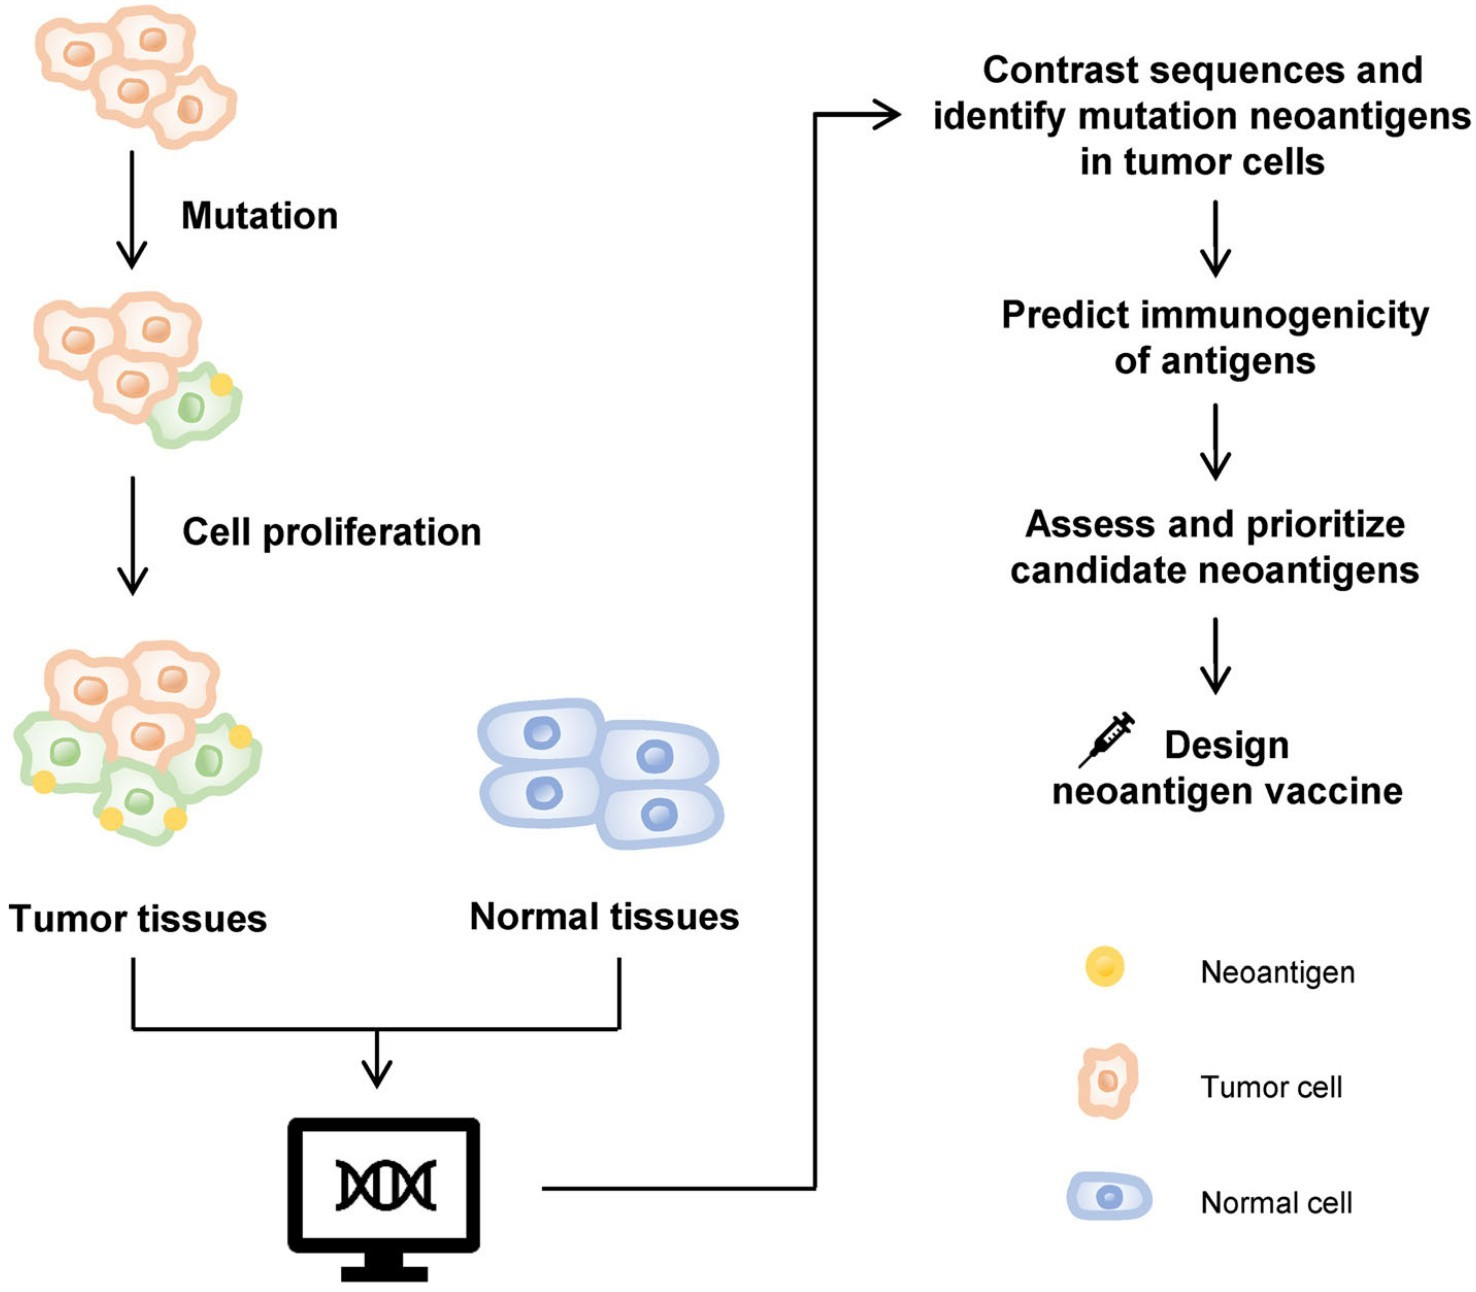
\includegraphics[width=0.6\textwidth]{img/neoantigen/process}
		\caption{Personalized vaccines process for Cancer \cite{peng2019neoantigen}.}
	\end{figure}		
\end{frame}
%-------------------------------------------------------
%-------------------------------------------------------



%-------------------------------------------------------
%-------------------------------------------------------
\begin{frame}{pMHC binding and presentation prediction}{}		
	\begin{figure}[H]
		\centering
		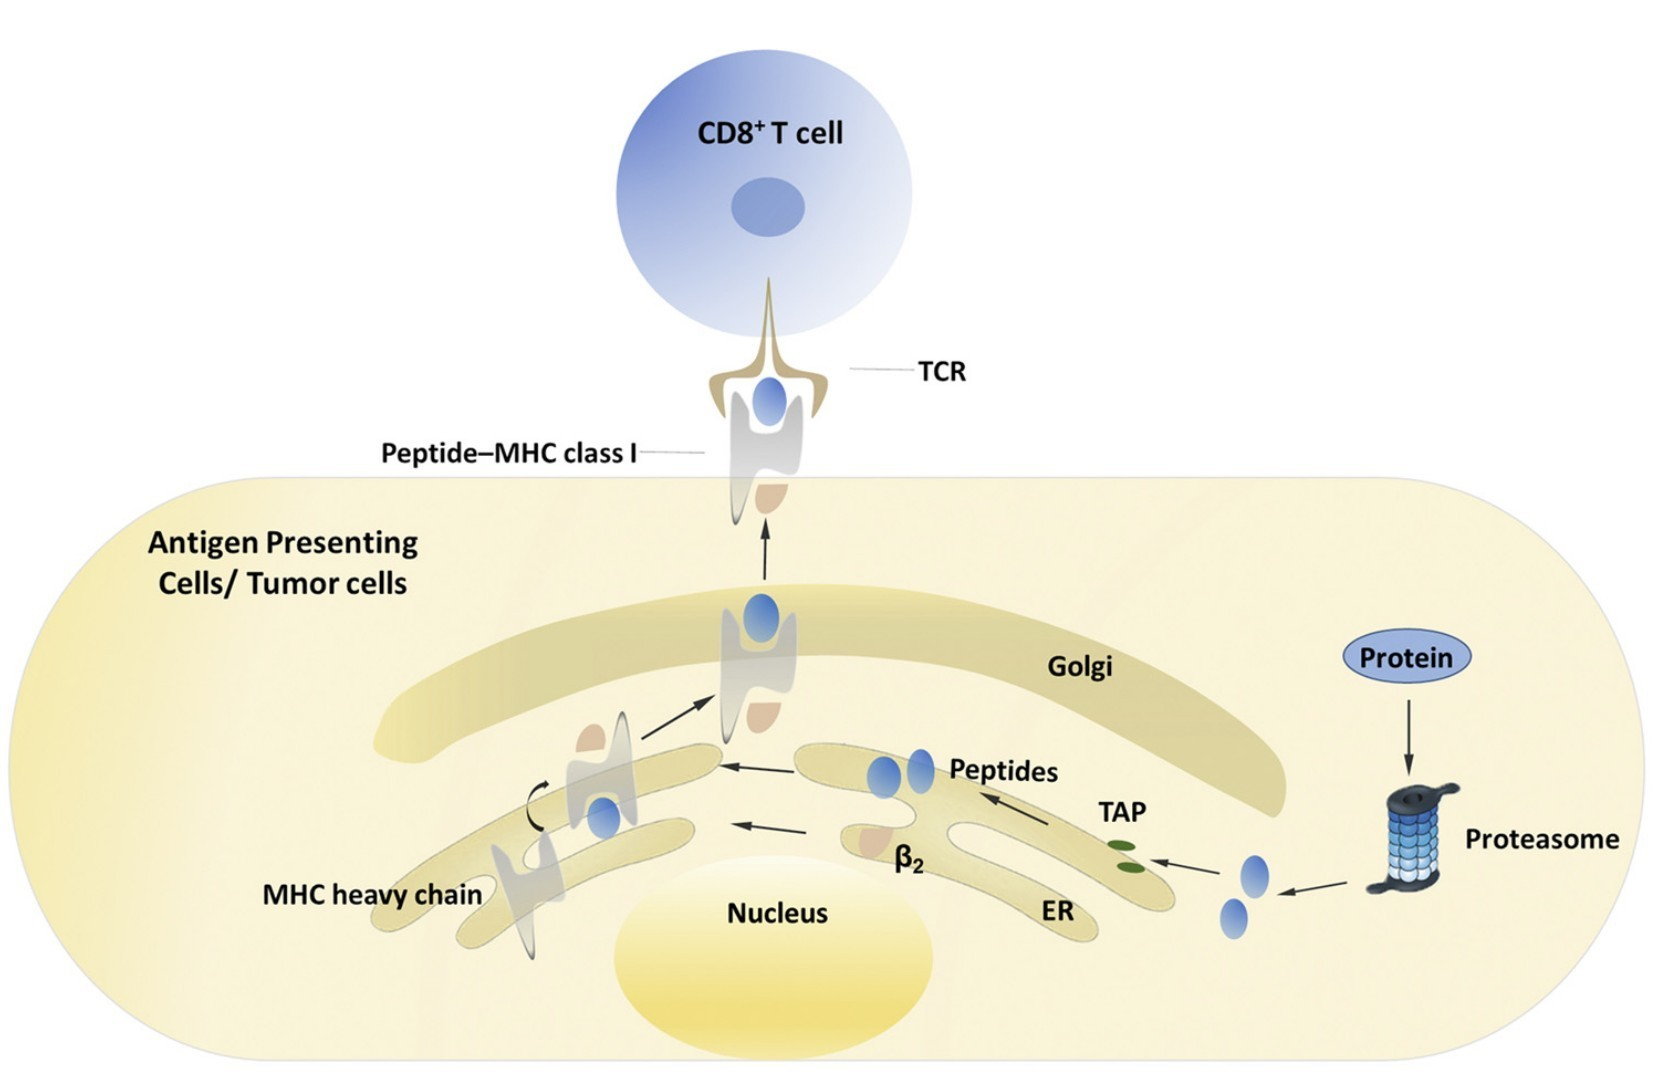
\includegraphics[width=0.9\textwidth]{img/neoantigen/mhc1.jpg}
		\caption{pMHC presentation process in MHC class I \cite{zhang2019application}.}
		\label{fig:mhc1}
	\end{figure}	
\end{frame}
%-------------------------------------------------------
%-------------------------------------------------------

%%%%%%%%%%%%%%%%%%%%%%%%%%%%%%%%%%%%%%%%%%%%%%%%%%%%%%%%%%%%%%%%%%%%%%%%%%%%%%%%%%%%%%%%%%%%%%%%%%%%%%%%%%%%%%%%
%%%%%%%%%%%%%%%%%%%%%%%%%%%%%%%%%%%%%%%%%%%%%%%%%%%%%%%%%%%%%%%%%%%%%%%%%%%%%%%%%%%%%%%%%%%%%%%%%%%%%%%%%%%%%%%%
%%%%%%%%%%%%%%%%%%%%%%%%%%%%%%%%%%%%%%%%%%%%%%%%%%%%%%%%%%%%%%%%%%%%%%%%%%%%%%%%%%%%%%%%%%%%%%%%%%%%%%%%%%%%%%%%
\subsection{Problem}
%%%%%%%%%%%%%%%%%%%%%%%%%%%%%%%%%%%%%%%%%%%%%%%%%%%%%%%%%%%%%%%%%%%%%%%%%%%%%%%%%%%%%%%%%%%%%%%%%%%%%%%%%%%%%%%%
%%%%%%%%%%%%%%%%%%%%%%%%%%%%%%%%%%%%%%%%%%%%%%%%%%%%%%%%%%%%%%%%%%%%%%%%%%%%%%%%%%%%%%%%%%%%%%%%%%%%%%%%%%%%%%%%
%%%%%%%%%%%%%%%%%%%%%%%%%%%%%%%%%%%%%%%%%%%%%%%%%%%%%%%%%%%%%%%%%%%%%%%%%%%%%%%%%%%%%%%%%%%%%%%%%%%%%%%%%%%%%%%%

%-------------------------------------------------------
%-------------------------------------------------------
\begin{frame}{Problem}{}
	
	\begin{block}{}
		\textbf{Less than 5\%} of detected neoantigens (peptides binded to MHC) succeed in activating the immune system \cite{de2020neoantigen}. Moreover, recent proposals only achieve 0.6 precision and 0.4 recall \cite{mill2022neoms}.
	\end{block}
			
			
	\begin{block}{}
		This is a \textbf{binary classification problem}. A peptide could be represented like: $p = \{ A, ... , Q \}$ and a MHC like: $q = \{ A, N, ... ,Q, E \}$. Finally, we need to know the probability of affinity between $p$ and $q$ (pMHC)
	\end{block}
	
%	\begin{block}{Objectives}
%		Proposed a method based on transformers and transfer learning for pMHC binding and	presentation prediction. 
%	\end{block}	
	
\end{frame}
%-------------------------------------------------------
%-------------------------------------------------------

%-------------------------------------------------------
%-------------------------------------------------------
\begin{frame}{Problem}{}	
	\begin{figure}
			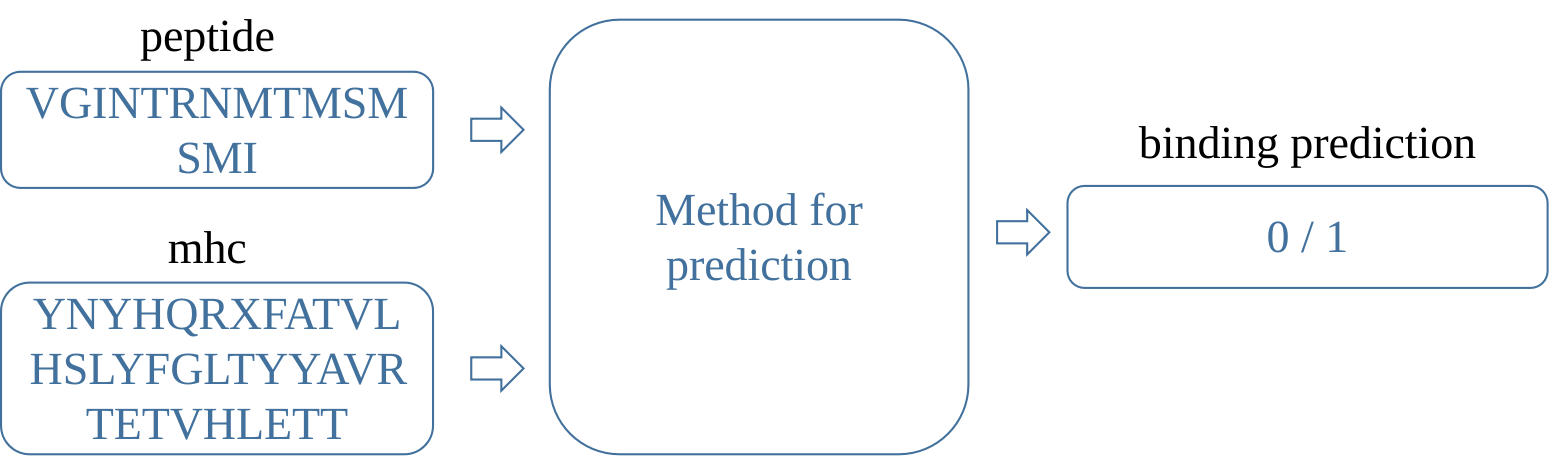
\includegraphics[width=0.97\textwidth]{img/neoantigen/problem}
			\caption{pMHC binding prediction problem.}
		\end{figure}
\end{frame}
%-------------------------------------------------------
%-------------------------------------------------------


%-------------------------------------------------------
%-------------------------------------------------------
%\begin{frame}{Objetivos}{}	
%	\begin{figure}
%		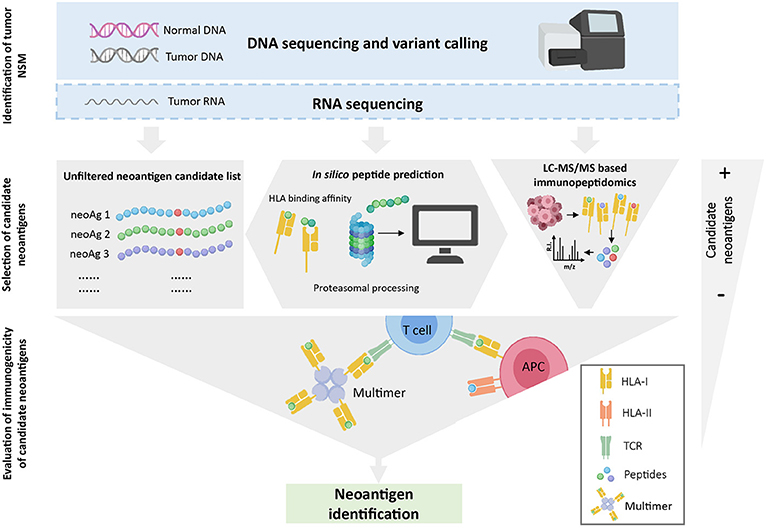
\includegraphics[width=0.97\textwidth]{img/neoantigen/pipeline_neoantigen}
		%\caption{Proceso de la detección de neo antígenos \cite{garcia2019determinants}.}
%	\end{figure}
%\end{frame}
%-------------------------------------------------------
%-------------------------------------------------------


%%%%%%%%%%%%%%%%%%%%%%%%%%%%%%%%%%%%%%%%%%%%%%%%%%%%%%%%%%%%%%%%%%%%%%%%%%%%%%%%%%%%%%%%%%%%%%%%%%%%%%%%%%%%%%%%
%%%%%%%%%%%%%%%%%%%%%%%%%%%%%%%%%%%%%%%%%%%%%%%%%%%%%%%%%%%%%%%%%%%%%%%%%%%%%%%%%%%%%%
\section{Related Works}
%%%%%%%%%%%%%%%%%%%%%%%%%%%%%%%%%%%%%%%%%%%%%%%%%%%%%%%%%%%%%%%%%%%%%%%%%%%%%%%%%%%%%%%%%%%%%%%%%%%%%%%%%%%%%%%%
%%%%%%%%%%%%%%%%%%%%%%%%%%%%%%%%%%%%%%%%%%%%%%%%%%%%%%%%%%%%%%%%%%%%%%%%%%%%%%%%%%%%%%


%-------------------------------------------------------
%-------------------------------------------------------
\begin{frame}{Related Works}{Transformers}
	
	\fontsize{8pt}{5pt}\selectfont
	
	\begin{table}[]
		\centering
		\caption{Recent works based on transformers and transfer learning.}		
		\setlength{\tabcolsep}{0.5em} % for the horizontal padding
		{\renewcommand{\arraystretch}{2}% for the vertical padding
			\begin{tabular}{p{0.6cm}p{0.6cm}p{2cm}p{5cm}}
				\textbf{Year} & \textbf{Ref.}                                  & \textbf{Name} & \textbf{Method}                                                                                                                                                                                                         \\ \hline
				2022 		  & \cite{zhang2022hlab} 		  &		\textbf{HLAB} 			 	   & Uses protBert model incascade with a RNN with attention  \\
				2022          & \cite{wang2022mhcroberta}     &     MHCRoBERTa           & Five encoders with 12 multiple-head self-attention pre-trainned with self-supervision             \\
				2022          & \cite{chu2022transformer}     &     \textbf{TransPHLA}             & Based on four modules: an embedding block, an encoder block (multiple self-attention), a feature optimization block (FC layer), and a projection block (FC layer used to predict)          \\
				2021          & \cite{cheng2021bertmhc}       &     BERTMHC             & Uses TAPE model followed by a linear layer.                          \\
				2021          & \cite{gasser2021interpreting} &     ImmunoBERT    	        & The same as BERTMHC focused on MHC-class I  \\
				
				           
			\end{tabular}
		}
	\end{table}	
\end{frame}
%-------------------------------------------------------
%-------------------------------------------------------


%%%%%%%%%%%%%%%%%%%%%%%%%%%%%%%%%%%%%%%%%%%%%%%%%%%%%%%%%%%%%%%%%%%%%%%%%%%%%%%%%%%%%%%%%%%%%%%%%%%%%%%%%%%%%%%%
%%%%%%%%%%%%%%%%%%%%%%%%%%%%%%%%%%%%%%%%%%%%%%%%%%%%%%%%%%%%%%%%%%%%%%%%%%%%%%%%%%%%%%
\section{Proposal}
%%%%%%%%%%%%%%%%%%%%%%%%%%%%%%%%%%%%%%%%%%%%%%%%%%%%%%%%%%%%%%%%%%%%%%%%%%%%%%%%%%%%%%%%%%%%%%%%%%%%%%%%%%%%%%%%
%%%%%%%%%%%%%%%%%%%%%%%%%%%%%%%%%%%%%%%%%%%%%%%%%%%%%%%%%%%%%%%%%%%%%%%%%%%%%%%%%%%%%%



%-------------------------------------------------------
%-------------------------------------------------------
\begin{frame}{Proposal}{}

	\vspace{0.5cm}
	\begin{figure}[H]
		\centering
		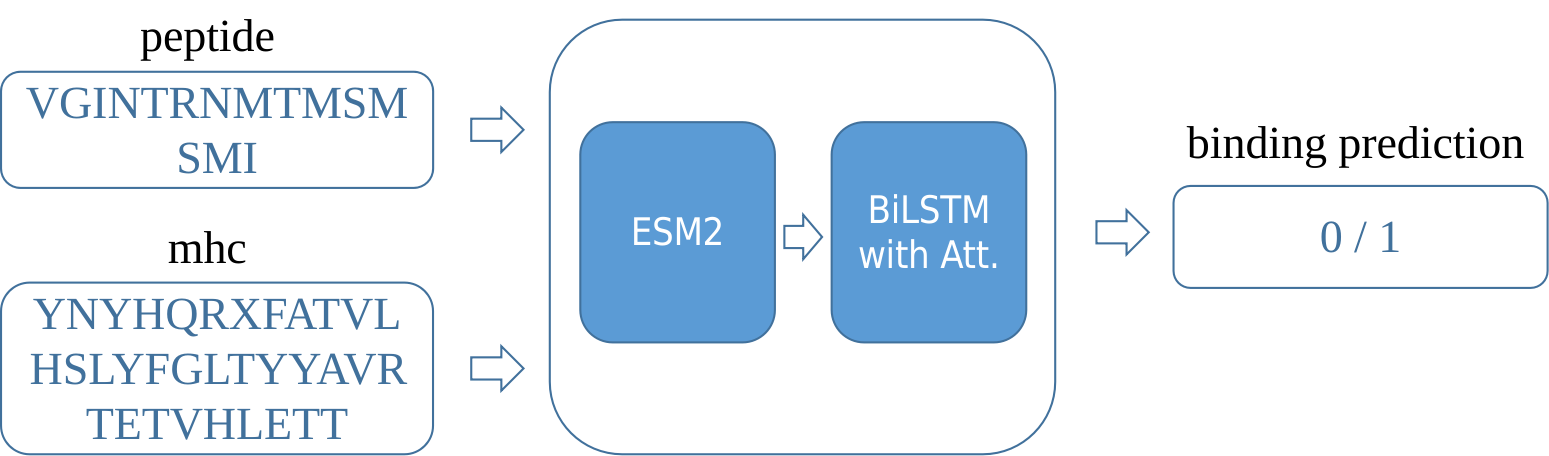
\includegraphics[width=0.9\textwidth]{img/neoantigen/proposal3}	
		\caption{Proposal for pMHC binding and presentation prediction.}
		\label{fig:neo_det_seq}
	\end{figure}
\end{frame}
%-------------------------------------------------------
%-------------------------------------------------------




%%%%%%%%%%%%%%%%%%%%%%%%%%%%%%%%%%%%%%%%%%%%%%%%%%%%%%%%%%%%%%%%%%%%%%%%%%%%%%%%%%%%%%%%%%%%%%%%%%%%%%%%%%%%%%%%
%%%%%%%%%%%%%%%%%%%%%%%%%%%%%%%%%%%%%%%%%%%%%%%%%%%%%%%%%%%%%%%%%%%%%%%%%%%%%%%%%%%%%%
\section{Preliminary Results}
%%%%%%%%%%%%%%%%%%%%%%%%%%%%%%%%%%%%%%%%%%%%%%%%%%%%%%%%%%%%%%%%%%%%%%%%%%%%%%%%%%%%%%%%%%%%%%%%%%%%%%%%%%%%%%%%
%%%%%%%%%%%%%%%%%%%%%%%%%%%%%%%%%%%%%%%%%%%%%%%%%%%%%%%%%%%%%%%%%%%%%%%%%%%%%%%%%%%%%%

%%%%%%%%%%%%%%%%%%%%%%%%%%%%%%%%%%%%%%%%%%%%%%%%%%%%%%%%%%%%%%%%%%%%%%%%%%%%%%%%%%%%%%%%%%%%%%%%%%%%%%%%%%%%%%%%
%%%%%%%%%%%%%%%%%%%%%%%%%%%%%%%%%%%%%%%%%%%%%%%%%%%%%%%%%%%%%%%%%%%%%%%%%%%%%%%%%%%%%%
\subsection{Models and databases}
%%%%%%%%%%%%%%%%%%%%%%%%%%%%%%%%%%%%%%%%%%%%%%%%%%%%%%%%%%%%%%%%%%%%%%%%%%%%%%%%%%%%%%%%%%%%%%%%%%%%%%%%%%%%%%%%
%%%%%%%%%%%%%%%%%%%%%%%%%%%%%%%%%%%%%%%%%%%%%%%%%%%%%%%%%%%%%%%%%%%%%%%%%%%%%%%%%%%%%%

%-------------------------------------------------------
%-------------------------------------------------------
\begin{frame}{Databases}{}
	
	We used the dataset from NetMHCIIpan3.2 \cite{jensen2018improved}.
	
	\begin{table}[h]
		\centering
		\caption{Samples used in training, evaluation and testing.}
		\setlength{\tabcolsep}{0.8em} % for the horizontal padding
		{\renewcommand{\arraystretch}{1.3}% for the vertical padding

		 	\begin{tabular}{ll}
		 		& \textbf{Samples}\\ \hline
		 		\textbf{Train}      & 107424        \\
		 		\textbf{Validation} & 13428        \\
		 		\textbf{Testing}    & 13429       
		 	\end{tabular}

		}
	\end{table}

\end{frame}
%-------------------------------------------------------
%-------------------------------------------------------

%-------------------------------------------------------
%-------------------------------------------------------
\begin{frame}{Models}{}
	
	Instead of ESM2 \cite{lin2023evolutionary} model, we used TAPE \cite{rao2019evaluating} because it is smaller and easier to train. Moreover, the Bi-LSTM with attention layer is based on HLAB \cite{zhang2022hlab}.
	
	\begin{table}[h]
		\centering
		\caption{Models used in experiments.}
		\setlength{\tabcolsep}{0.8em} % for the horizontal padding
		{\renewcommand{\arraystretch}{1.3}% for the vertical padding
			
			\begin{tabular}{lp{6cm}}
				& \textbf{Description}\\ \hline
				\textbf{BERTMHC-LINEAR}      & BERT architecture followed by a linear layer        \\
				\textbf{BERTMHC-RNN} & BERT architecture followed by a BiLSTM layer and then a Linear layer        \\
				\textbf{BERTMHC-RNN-ATT}    & BERT architecture followed by a BiLSTM layer with attention and then a Linear layer       
			\end{tabular}
			
		}
	\end{table}
	
\end{frame}
%-------------------------------------------------------
%-------------------------------------------------------


%%%%%%%%%%%%%%%%%%%%%%%%%%%%%%%%%%%%%%%%%%%%%%%%%%%%%%%%%%%%%%%%%%%%%%%%%%%%%%%%%%%%%%%%%%%%%%%%%%%%%%%%%%%%%%%%
%%%%%%%%%%%%%%%%%%%%%%%%%%%%%%%%%%%%%%%%%%%%%%%%%%%%%%%%%%%%%%%%%%%%%%%%%%%%%%%%%%%%%%
\subsection{Comparison}
%%%%%%%%%%%%%%%%%%%%%%%%%%%%%%%%%%%%%%%%%%%%%%%%%%%%%%%%%%%%%%%%%%%%%%%%%%%%%%%%%%%%%%%%%%%%%%%%%%%%%%%%%%%%%%%%
%%%%%%%%%%%%%%%%%%%%%%%%%%%%%%%%%%%%%%%%%%%%%%%%%%%%%%%%%%%%%%%%%%%%%%%%%%%%%%%%%%%%%%

%-------------------------------------------------------
%-------------------------------------------------------
\begin{frame}{Training}{}

	\begin{figure}[H]
		\centering
		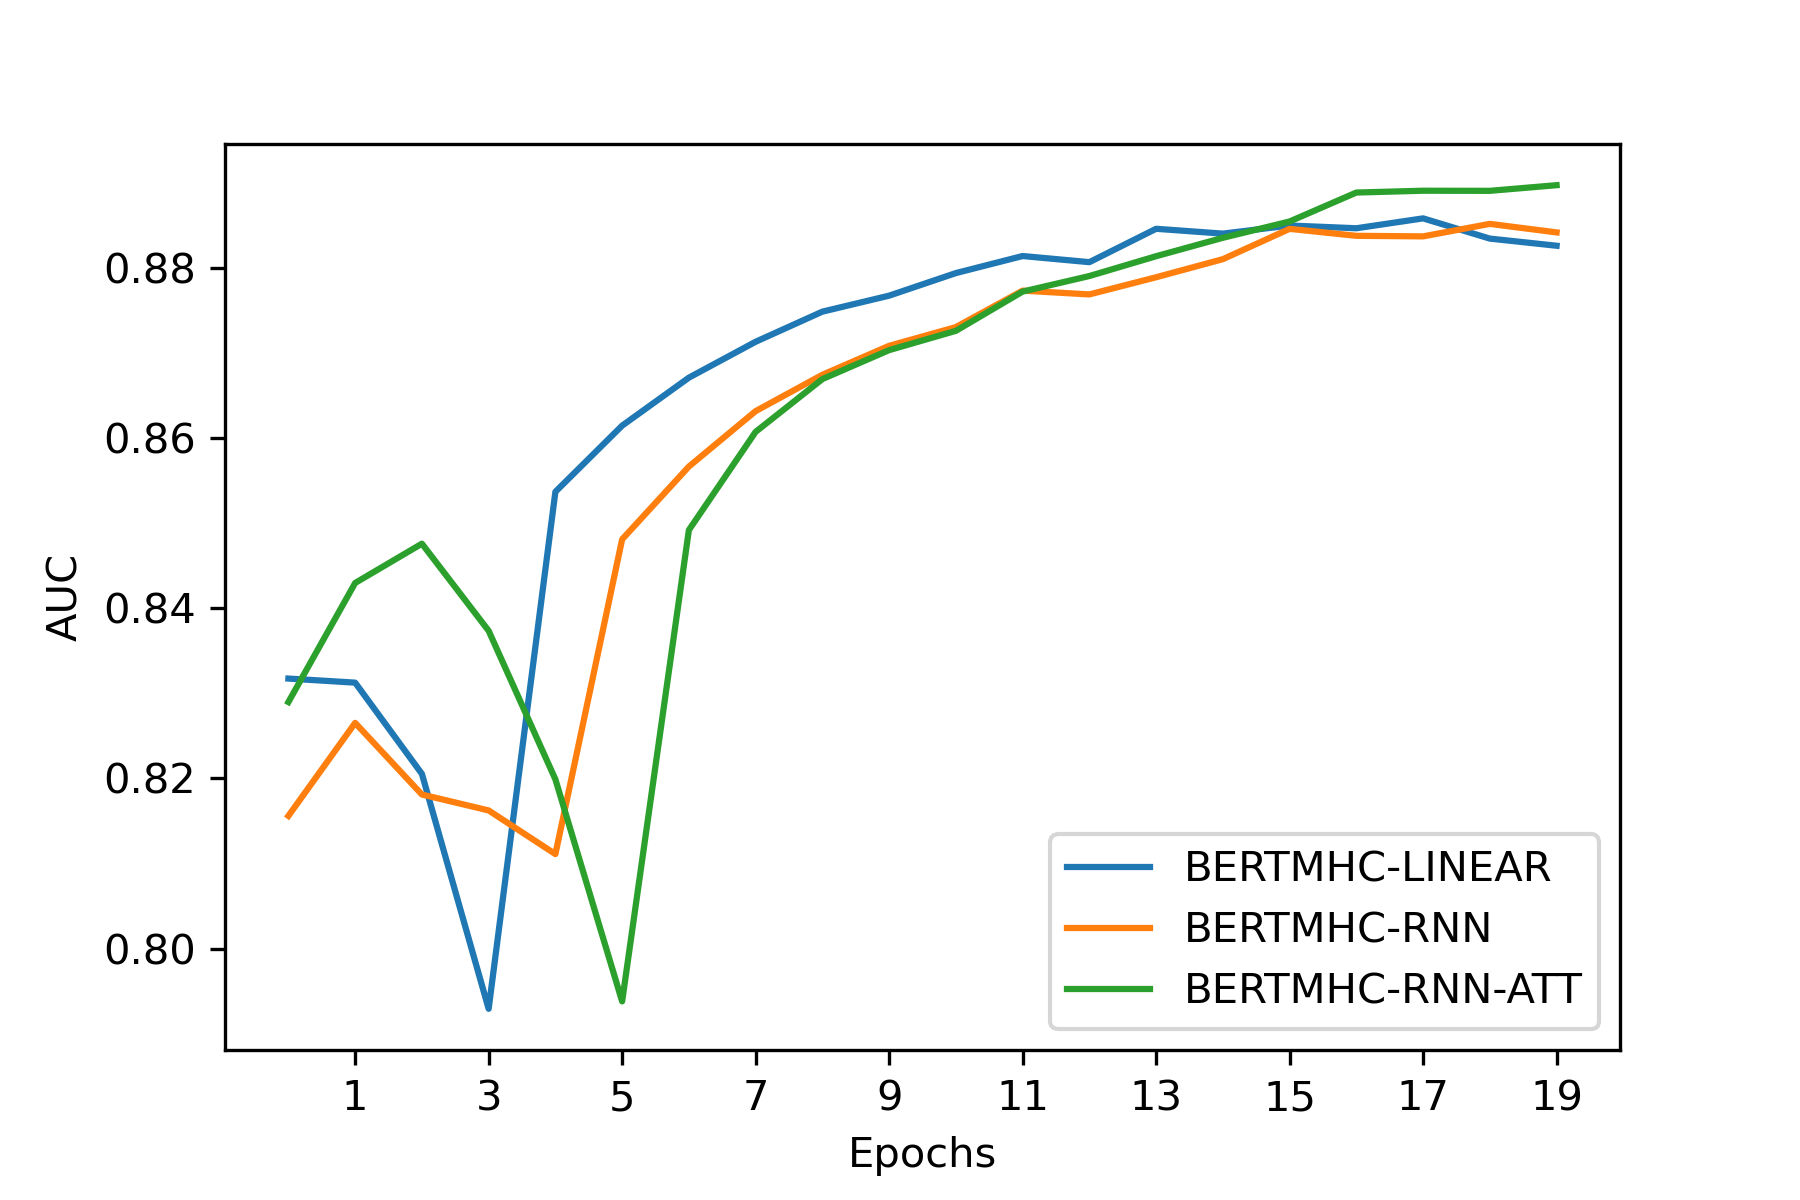
\includegraphics[width=0.8\textwidth]{img/metrics/training_3_7_8}	
		\caption{AUC per epoch of models.}		
	\end{figure}
\end{frame}
%-------------------------------------------------------
%-------------------------------------------------------

%-------------------------------------------------------
%-------------------------------------------------------
\begin{frame}{Comparison}{}

	\begin{figure}[H]
		\centering
		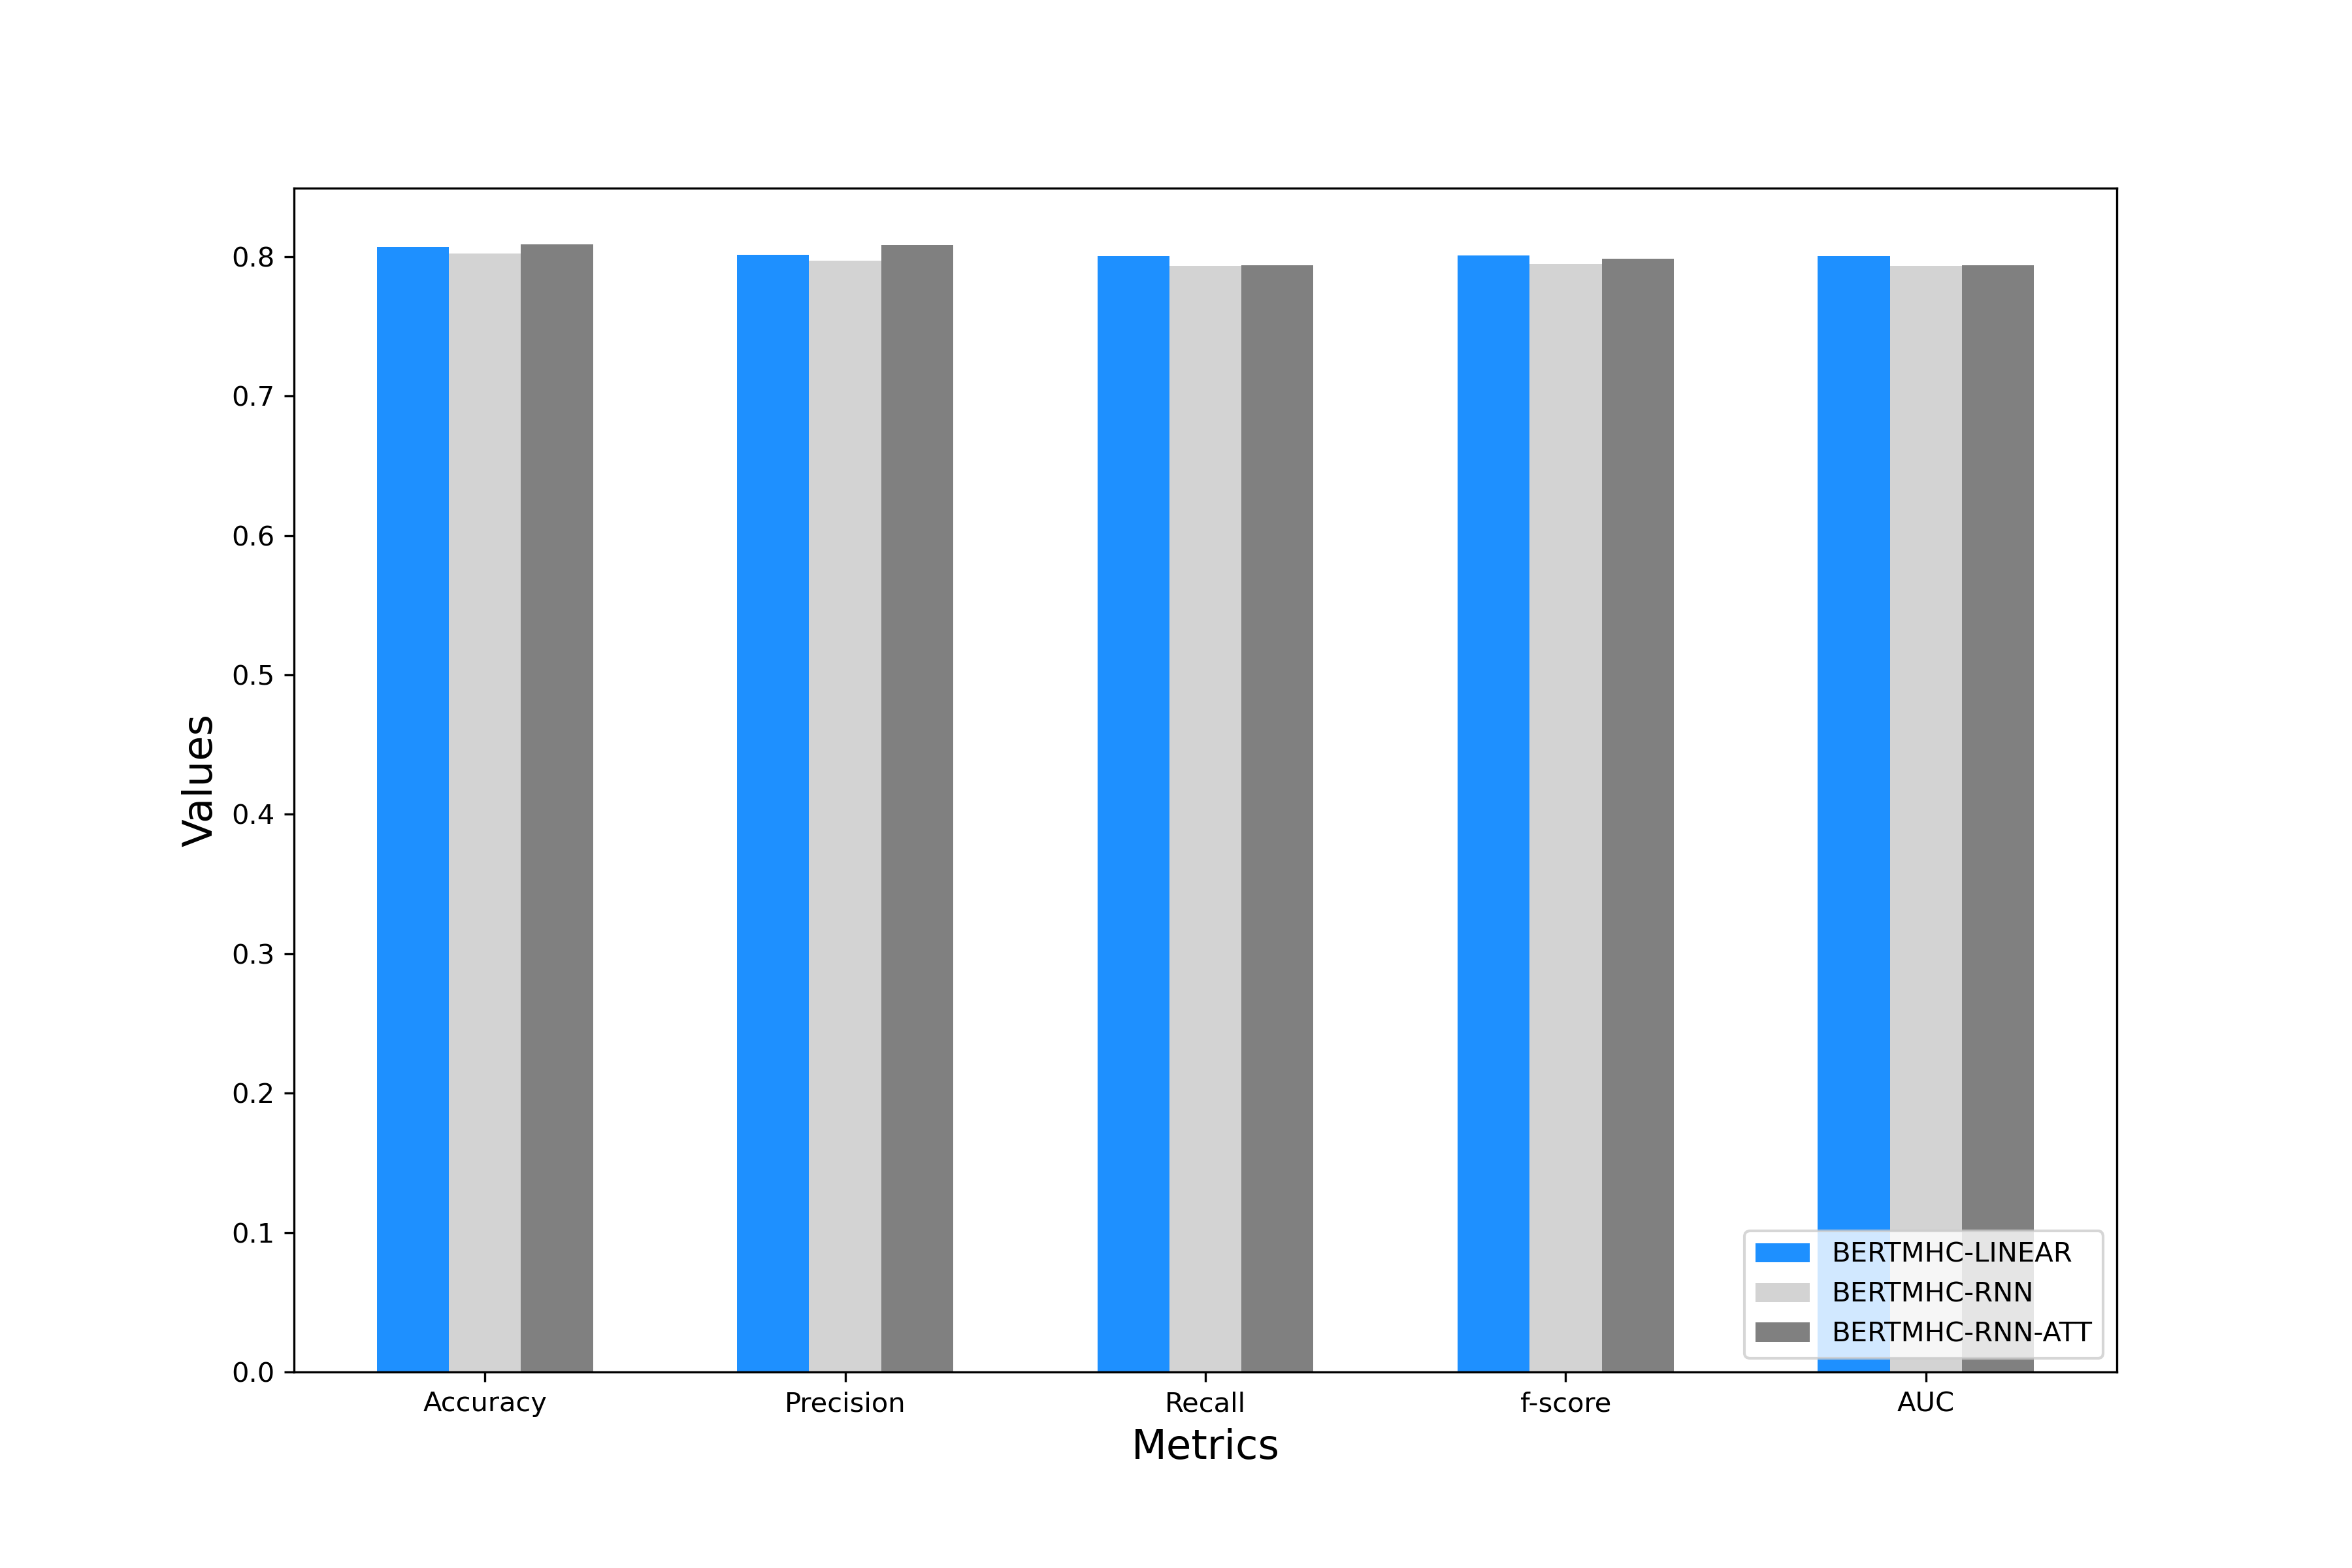
\includegraphics[width=0.8\textwidth]{img/metrics/metrics_comparison_3_7_8}	
		\caption{Metrics comparison.}		
	\end{figure}
\end{frame}
%-------------------------------------------------------
%-------------------------------------------------------

%-------------------------------------------------------
%-------------------------------------------------------
\begin{frame}{Comparison}{}
	
\begin{table}[]
	\caption{Metrics comparison of BERTMHC-LINEAR, BERTMHC-RNN and BERTMHC-RNN-ATT}
	\setlength{\tabcolsep}{0.8em} % for the horizontal padding
	{\renewcommand{\arraystretch}{1.3}% for the vertical padding
	\begin{tabular}{llllll}
		\textbf{Model} & \textbf{Acc} & \textbf{Precision} & \textbf{Recall} & \textbf{Fscore} & \textbf{AUC} \\ \hline
		LINEAR & 0.8070       & 0.8012             & \textbf{0.8005}          & \textbf{0.8009}          & \textbf{0.8005}       \\
		RNN & 0.8023       & 0.7972             & 0.7932          & 0.7949          & 0.7932       \\
		RNN-ATT & \textbf{0.8086}       & \textbf{0.8082}             & 0.7937          & 0.7985          & 0.7937      
	\end{tabular}
}
\end{table}
\end{frame}
%-------------------------------------------------------
%-------------------------------------------------------



%-------------------------------------------------------
%-------------------------------------------------------
\begin{frame}{Comparison}{}
	\begin{figure}[H]
		\centering
		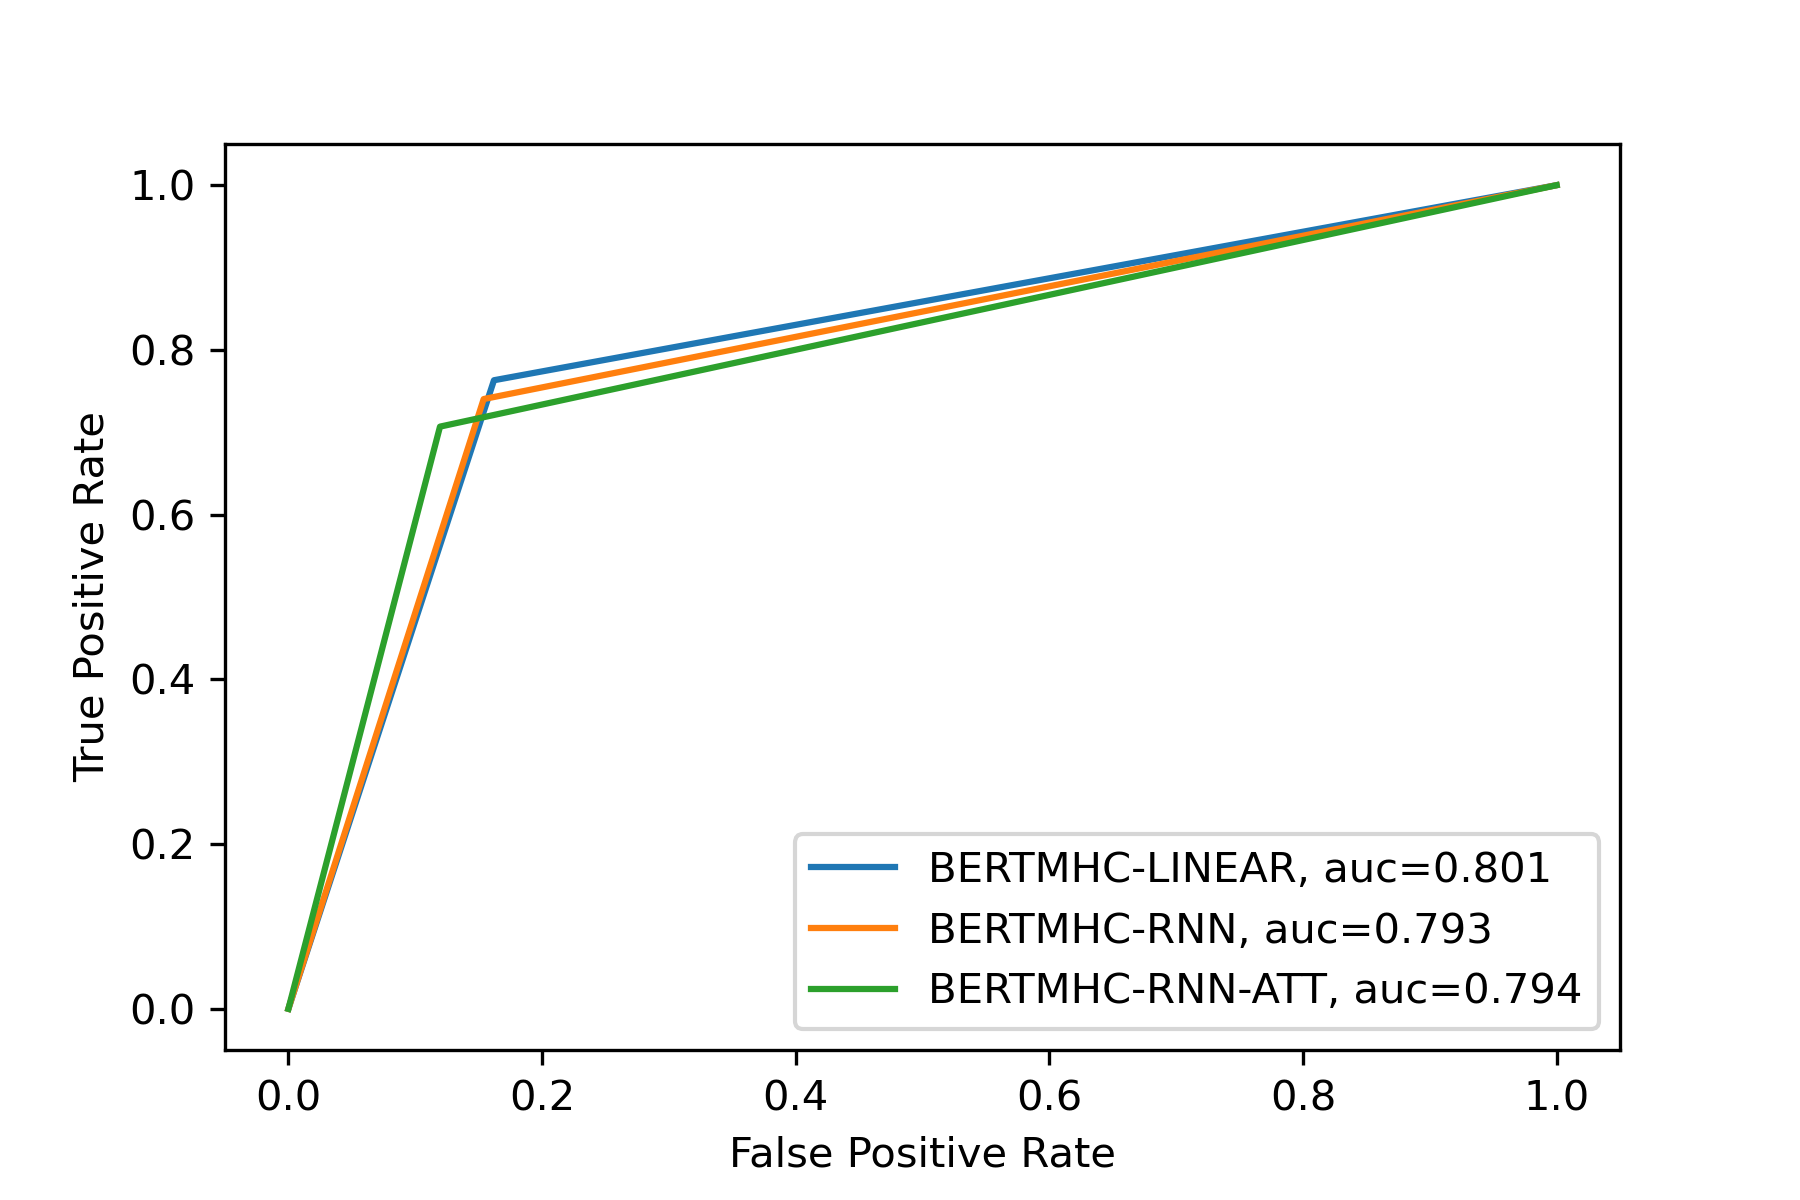
\includegraphics[width=0.8\textwidth]{img/metrics/roc_comparison_3_7_8}	
		\caption{ROC curve.}		
	\end{figure}
\end{frame}
%-------------------------------------------------------
%-------------------------------------------------------




%%%%%%%%%%%%%%%%%%%%%%%%%%%%%%%%%%%%%%%%%%%%%%%%%%%%%%%%%%%%%%%%%%%%%%%%%%%%%%%%%%%%%%%%%%%%%%%%%%%%%%%%%%%%%%%%
%%%%%%%%%%%%%%%%%%%%%%%%%%%%%%%%%%%%%%%%%%%%%%%%%%%%%%%%%%%%%%%%%%%%%%%%%%%%%%%%%%%%%%
\section{Conclusions}
%%%%%%%%%%%%%%%%%%%%%%%%%%%%%%%%%%%%%%%%%%%%%%%%%%%%%%%%%%%%%%%%%%%%%%%%%%%%%%%%%%%%%%%%%%%%%%%%%%%%%%%%%%%%%%%%
%%%%%%%%%%%%%%%%%%%%%%%%%%%%%%%%%%%%%%%%%%%%%%%%%%%%%%%%%%%%%%%%%%%%%%%%%%%%%%%%%%%%%%


%-------------------------------------------------------
%-------------------------------------------------------
\begin{frame}{Conclusions}{}
	
	\begin{block}{}
		In this preliminary results, we evaluated a BERT architecture (transformer) with transfer learning from TAPE. We choose TAPE because, it is smaller and easier to train. In future experiments, we will evaluate ESM2.  
	\end{block}

	\begin{block}{}
		According to experiments, BERTMHC-LINEAR and BERTMHC-RNN-ATT got better results in netMHCIIpan3.2 dataset. This happens, because we evaluated these models in a small dataset. In future experiments, we will evaluated these models in a larger dataset. 
	\end{block}

\end{frame}
%-------------------------------------------------------
%-------------------------------------------------------


%-------------------------------------------------------
%-------------------------------------------------------
\begin{frame}[allowframebreaks]
	\frametitle{References}
	%\bibliographystyle{amsalpha}
	\bibliographystyle{IEEEtran}
	\bibliography{Bibliography.bib}
\end{frame}
%-------------------------------------------------------
%-------------------------------------------------------

%-------------------------------------------------------
%-------------------------------------------------------
\if\mycmd1 % MY THEME
\1{
	{\1
		\begin{frame}[plain,noframenumbering]
			%\finalpage{Thank you}
			\begin{figure}[]
				\centering
				
\includegraphics[width=\textwidth,height=0.7\textheight,keepaspectratio]{img/question.png}
				%\label{img:mot2}
				%\caption{Image example in 2 gray levels.}
			\end{figure}
	\end{frame}}
	\else % CS THEME
	\begin{frame}{Questions?}
		\begin{figure}[]
			\centering
			
\includegraphics[width=\textwidth,height=0.7\textheight,keepaspectratio]{img/question.png}
			%\label{img:mot2}
			%\caption{Image example in 2 gray levels.}
		\end{figure}
		
	\end{frame}
	\fi
	%-------------------------------------------------------
	%-------------------------------------------------------
	

\end{document}